\chapter{Design}
\label{sec:design}

% Ist das zentrale Kapitel der Arbeit. Hier werden das Ziel sowie die
% eigenen Ideen, Wertungen, Entwurfsentscheidungen vorgebracht. Es kann
% sich lohnen, verschiedene Möglichkeiten durchzuspielen und dann
% explizit zu begründen, warum man sich für eine bestimmte entschieden
% hat. Dieses Kapitel sollte - zumindest in Stichworten - schon bei den
% ersten Festlegungen eines Entwurfs skizziert werden.
% Es wird sich aber in einer normal verlaufenden
% Arbeit dauernd etwas daran ändern. Das Kapitel darf nicht zu
% detailliert werden, sonst langweilt sich der Leser. Es ist sehr
% wichtig, das richtige Abstraktionsniveau zu finden. Beim Verfassen
% sollte man auf die Wiederverwendbarkeit des Textes achten.

% Plant man eine Veröffentlichung aus der Arbeit zu machen, können von
% diesem Kapitel Teile genommen werden. Das Kapitel wird in der Regel
% wohl mindestens 8 Seiten haben, mehr als 20 können ein Hinweis darauf
% sein, daß das Abstraktionsniveau verfehlt wurde.

%\ldots design \ldots

%\todo{write design}

This chapter analyzes the system call implementation and other 
IO methods used to communicate between applications 
and user-level processes. Based on the various deficiencies of the 
traditional methods, we will propose a novel mechanism, which is aim 
to improve the IO performance and secure the isolation 
between applications and devices.


\begin{figure}[H]
  \centering
  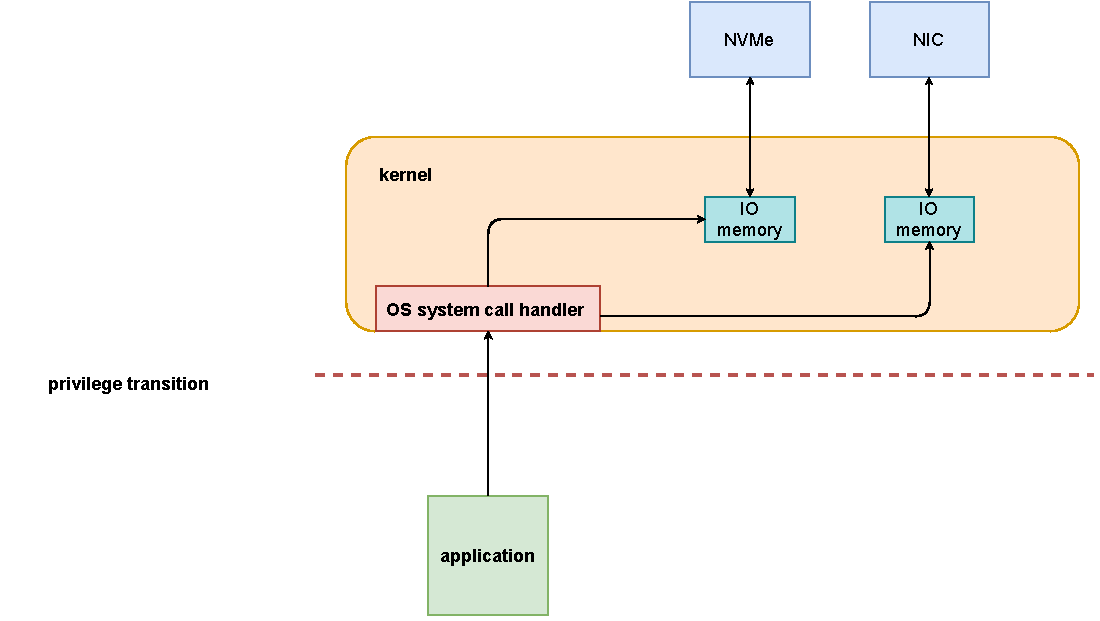
\includegraphics[width=0.8\textwidth]{images/system_call_path_design_3}
  \caption[Short description]{System call workflow}
  \label{fig:system_call_path_design_3}
\end{figure}

\section{Kernel Offloading}
Figure ~\ref{fig:system_call_path_design_3} shows that the application must enter the kernel 
to interact with devices with the help of system calls. 
Due to security issues, OS exploits ring protection to isolate 
applications and devices since applications are not trustworthy. 
With the continuous improvement of IO performance requirements 
from applications in recent years, this mechanism is becoming outdated. 
The main reason comes from the kernel and its side effect. Specifically, 
the networking stack in the kernel is designed for the compatibility of 
variant network protocols instead of high-performance communication. 
In addition, the privilege transitions between the user space and kernel 
is very costly. Therefore, the speed of IO paths through the kernel is slow.

How to address this issue? The most straightforward 
answer is kernel bypass. Kernel bypass allows applications to directly 
communicate with devices by mapping the device registers into user space. 
Hint, severe performance penalty caused by the kernel is dropped. 
The application could manipulate device registers similar to accessing memory. 
In addition, through configuring device registers, data can be 
transferred directly between application and device using \verb|DMA|, 
instead of copying it multiple times, i.e., NIC to the kernel, 
the kernel to user land applications.

In summary, Mapping devices to user space has two advantages. 
The first is that the performance is increased dramatically 
by avoiding privilege transitions. Secondly, multiple copies 
between applications and devices can be avoided. 
Hence, we would like to map device registers to user space 
in our fast call mechanism too

\section{Isolation Between User And Device}



Directly mapping device registers to user space 
is faster for communication between applications 
and devices. However, it could be a disaster in terms 
of security. Imagine that if an attacker knows where device
 registers are, he can intentionally manipulate the device, 
 leading to a device crash. More serious is that the attacker 
 can intercept other applications' packages or send wrong messages to others.  
Hence, the fast call mechanism needs isolation between application 
and device registers in some degradation. 

\begin{figure}[tbp]
  \centering
  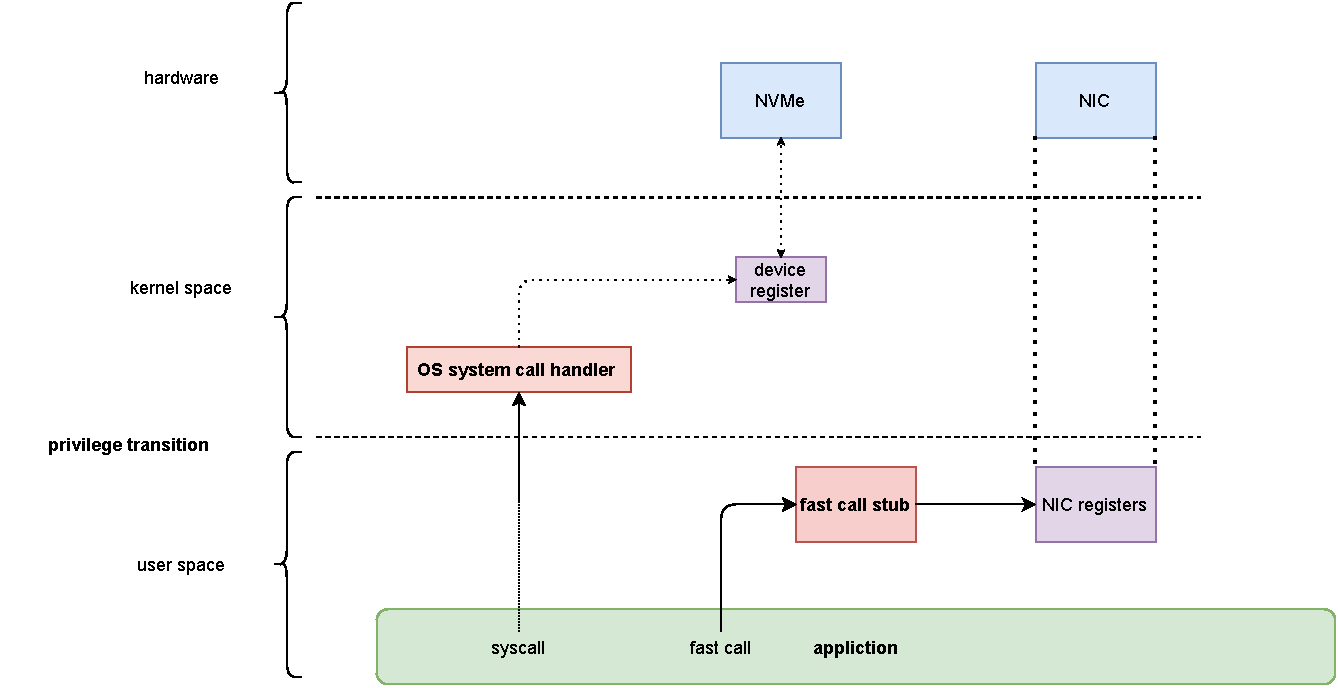
\includegraphics[width=0.8\textwidth]{images/fast_call_design_idea1}
  \caption[Short description]{Fast call design idea}
  \label{fig:fast_call_design_idea1}
\end{figure}

The fast call mechanism uses two methods to isolate the 
device registers from the application. First,  the memory 
address of device registers should be random, and the 
application should not know the registers' location. 
This makes it hard for an attacker to guess where the 
registers are and gain control of devices.  In addition, 
as shown in figure ~\ref{fig:fast_call_design_idea1}, The 
fast call mechanism places a stub between the application 
and device registers. The stub contains the location of device 
registers and code that defines what the application can do on 
the device. In particular, this stub is only executable, which 
means an application cannot either read the location of device 
registers out of this stub or change the code in the stub. 
The application can only call the stub and complete the predefined 
operation on the device registers based on the stub's code. 	 

\section{Flexibility}
In short, every fast call is composed of two parts: the only 
executable stub and user space mapped device registers. 
By doing so, we could isolate devices from an untrustworthy 
application successfully. 

As we analyzed before, an application exploits the 
\verb|SYSCALL| instruction to invoke a system call. 
Compared with the system call, after an application has 
registered a fast call through IOCTL, it can directly call 
the fast call through the function pointer. We will discuss 
in detail the fast call's registration process in the following 
chapters. For now, you only need to know that fast call infrastructure 
returns the stub address to the application after a fast 
call registration is complete.  The application can use a 
function pointer to the stub to invoke the fast call. Thus, 
invoking a fast is similar to a regular function call which 
means it is very flexible and easy to integrate into the 
user-level implementation.

\begin{figure}[tbp]
  \centering
  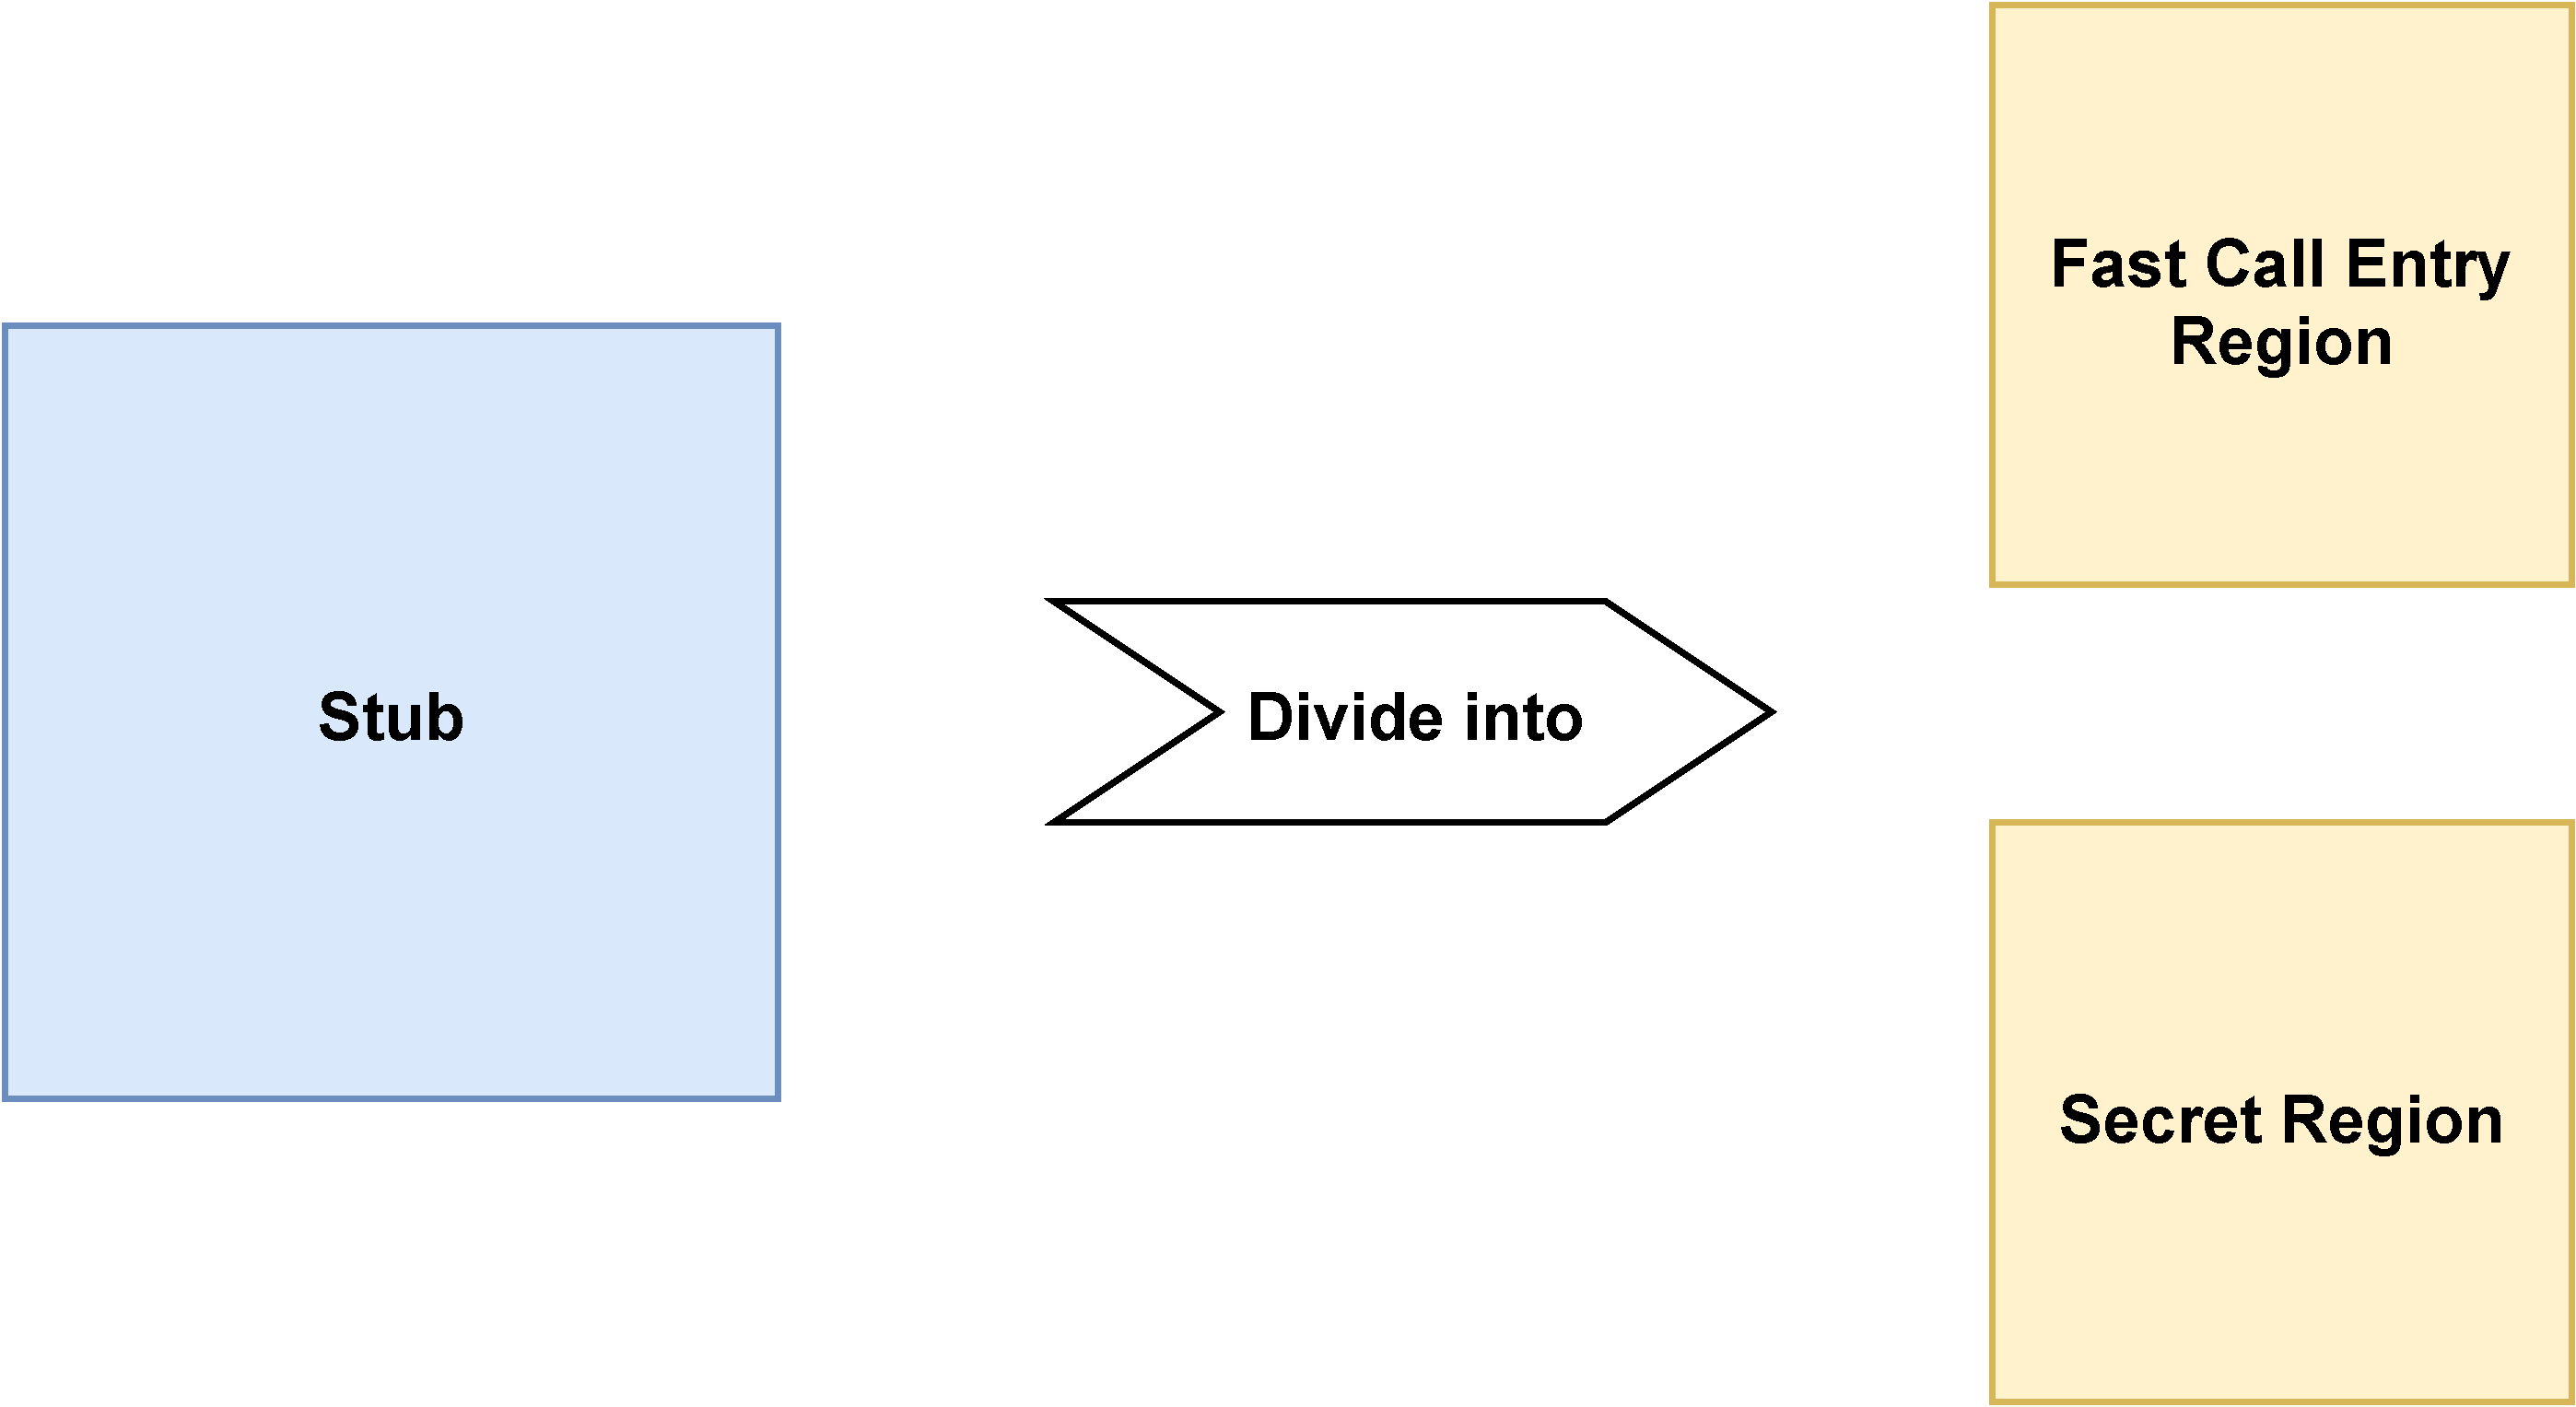
\includegraphics[width=0.8\textwidth]{images/Stub_partition}
  \caption[Short description]{Stub Partition}
  \label{fig:Stub_partition}
\end{figure}

Let us go a bit dipper to the stub in a fast call. 
In order to facilitate understanding, we mentioned that this 
stub is only executable. However, this statement is partially correct. 

An application needs the stub to be readable to invoke 
the fast call through a function pointer to the code on 
the stub. The reason is that using a function pointer requires 
that the code pointed by the pointer is located on a readable 
and executable memory region. On the other hand, we need the 
memory region of the stub only executable to prevent an attacker 
from reading secrets(devices' location) stored on the stub. 
How to solve this conflict? The answer is simple: separate the 
stub into two parts, i.g., the fast call entry and the secret regions. 
As shown in the figure  ~\ref{fig:Stub_partition}, the fast 
call entry region contains the code predefined how to manipulate 
the device registers, and this region is executable and readable. 
The fast call second region contains the secrets(location of device 
registers on user space) and is an executable memory region. 
Note that the fast call entry region does not know the secrets, 
which means that the entry region needs to retrieve the secrets 
from the secret region if it wants to manipulate the device registers.
Finally, remember previously, a fast call is invoked by a function 
pointer to the stub in the fast call?  Due to the stub being divided 
into the fast call entry and secret region, a fast call needs to be 
invoked by the function pointer to the fast call entry region.
\section{Overview}
\begin{figure}[tbp]
  \centering
  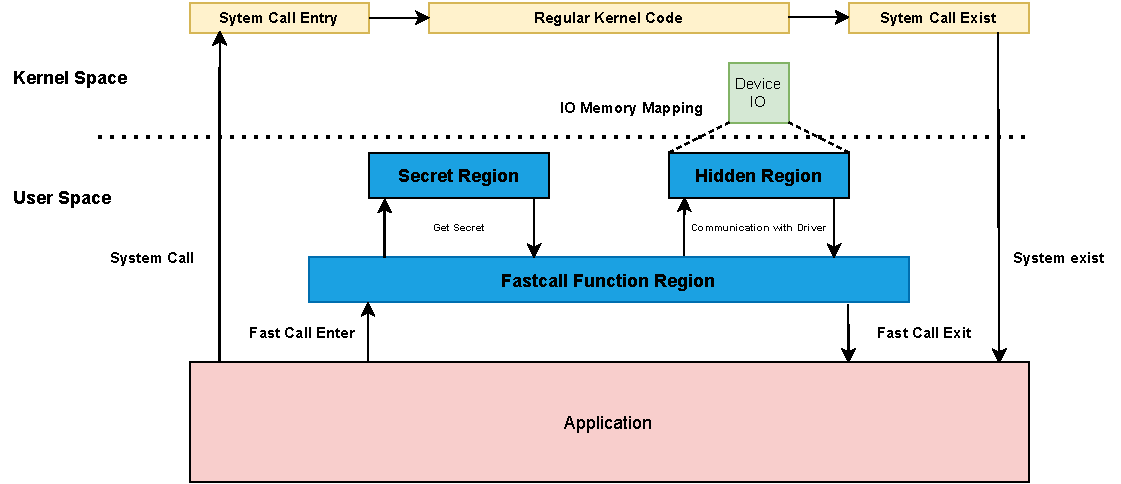
\includegraphics[width=0.8\textwidth]{images/fastcall_architecture}
  \caption[Short description]{Fast call Architecture}
  \label{fig:fastcall_architecture}
\end{figure}



So far, we have learned multiple design decisions of the fast call. 
Now let us take a look at the overview of the fast call. Generally, 
a fast call is running in the user space(non-privileged level) and is 
composed of 3 parts, i.e., the entry region, the secret region, and the 
device registers mapped to user space. 	In the following discussion, 
we name the device registers mapped to the user space as hidden regions.

Figure ~\ref{fig:fastcall_architecture} illustrates the 
architecture of the fast system call mechanism in the current 
version. The core of each fast call is composed of 3 different 
memory regions. They are the fast call entry, secret, and hidden region. 
In order to distinguish between system calls and fast calls, these two 
mechanisms have different calling methods. Compared to the system call, 
an application uses a function pointer to the entry region returned by 
the fast call registration function to call the fast call. Because all 
the components of a fast call run in the user space, the application can 
use fast calls like a typical function call and avoid performance 
loss in system calls.

The fast call entry region is the core of a fast call. 
It is a memory area that is readable and executable and 
contains the code for the fast call. The code on this 
region assumes the responsibility of the service function 
in the system call mechanism. It completes all predefined 
operations on device registers in hidden regions and returns 
the result to an application. Specifically, this code verifies 
the parameters passed in by the application, retrieves secrets 
from the secret region, and manipulates devices. 

The secret region contains addresses of the hidden region as secrets. 
The secret region's unique feature is that it is only an executable memory 
area in user space. Thus, any attempt to read the content in this region 
will cause an exception. In this way, we protected the secrets in this 
region from attackers.

The hidden region is the device registers mapped on user space. 
A fast call could directly manipulate a device through this region 
without the privilege transition. Note that a fast call may have 
multiple hidden regions since a device may have multiple registers 
and fast call support map those register into different places. 
To protect this region from attack, we randomize fast call's 
each hidden region during the fast call registration process. 
Thus, there is a high chance that the fast call entry region 
can access hidden regions.

In short, we introduced a new communication mechanism between 
application and device to increase the IO performance. 
The next chapter will introduce the implementation details 
of this new mechanism and how to register for fast calls.
\cleardoublepage

%%% Local Variables:
%%% TeX-master: "diplom"
%%% End:
